\documentclass[12pt,twoside]{article}

%\documentclass[a4paper,10pt,twoside]{article}
\usepackage{amsmath,amsfonts,amssymb}
\usepackage{ucs}  % Unicode support
\usepackage[utf8x]{inputenc}
\usepackage{culmus}
%\usepackage{float}
%\usepackage{listings}
\usepackage{color} %red, green, blue, yellow, cyan, magenta, black, white
\definecolor{mygreen}{RGB}{28,172,0} % color values Red, Green, Blue
\definecolor{mylilas}{RGB}{170,55,241}

%\usepackage[cp1255]{inputenc}
\usepackage[english,hebrew]{babel}
%BIDION

%\usepackage{xkeyval}
\usepackage{graphicx}

\usepackage{epstopdf}
%\usepackage{eucal}
%\usepackage{mathrsfs}
%\usepackage{theorem}
%\usepackage{pifont}
\usepackage {epsfig}
%\usepackage[colorlinks=true, bookmarks=true]{hyperref}
\usepackage{bibtopic,wrapfig}
%\usepackage{bbding}
%\usepackage{fancyhdr}
%\usepackage{verbatim}

%\pagestyle{fancy}

%\usepackage{bidi}


%\rhead{\thepage}
%\lfoot{\small \copyright\;\;\; שירה בר-דב, אורט בראודה}
%\rfoot{\thepage}
%\cfoot{}
%\renewcommand{\headrulewidth}{0.4pt}
%\renewcommand{\footrulewidth}{0.4pt}
%\DeclareGraphicsExtensions{.pdf,.png,.jpg}
%\let\arref\ref
%\renewcommand{\ref}[1]{\I{\arref{#1}}}

\setlength{\parskip}{6pt} \setlength{\parindent}{0pt}
\setlength{\oddsidemargin}{0pt} \setlength{\evensidemargin}{0pt}
%\documentclass[a4paper,10pt,twoside]{article}
\usepackage{amsmath,amsfonts,amssymb}
\usepackage{ucs}  % Unicode support
\usepackage[utf8x]{inputenc}
\usepackage{culmus}
%\usepackage{float}
%\usepackage{listings}
\usepackage{color} %red, green, blue, yellow, cyan, magenta, black, white
\definecolor{mygreen}{RGB}{28,172,0} % color values Red, Green, Blue
\definecolor{mylilas}{RGB}{170,55,241}

%\usepackage[cp1255]{inputenc}
\usepackage[english,hebrew]{babel}
%BIDION

%\usepackage{xkeyval}
\usepackage{graphicx}

\usepackage{epstopdf}
%\usepackage{eucal}
%\usepackage{mathrsfs}
%\usepackage{theorem}
%\usepackage{pifont}
\usepackage {epsfig}
%\usepackage[colorlinks=true, bookmarks=true]{hyperref}
\usepackage{bibtopic,wrapfig}
%\usepackage{bbding}
%\usepackage{fancyhdr}
%\usepackage{verbatim}

%\pagestyle{fancy}

%\usepackage{bidi}

% User packages
%%%%%%%%%%%%%%%%%%%%%%%%%%%%%%%%
\usepackage{subcaption}


%\rhead{\thepage}
%\lfoot{\small \copyright\;\;\; שירה בר-דב, אורט בראודה}
%\rfoot{\thepage}
%\cfoot{}
%\renewcommand{\headrulewidth}{0.4pt}
%\renewcommand{\footrulewidth}{0.4pt}
%\DeclareGraphicsExtensions{.pdf,.png,.jpg}
%\let\arref\ref
%\renewcommand{\ref}[1]{\I{\arref{#1}}}

\setlength{\parskip}{2em} \setlength{\parindent}{0pt}
\setlength{\oddsidemargin}{0pt} \setlength{\evensidemargin}{0pt}

% User defined macros
%%%%%%%%%%%%%%%%%%%%%%%%%%%%%%%%

\newtheorem{definition}{הגדרה}[section]
\newtheorem{theorem}{משפט}[section]
\newtheorem{proposition}{טענה}[section]
\newtheorem{conjecture}{השערה}[section]
\newtheorem{corollary}{מסקנה}[section]
\newtheorem{lemma}{למה}[section]
\newtheorem{question}{שאלה}[section]
\newtheorem{example}{דוגמה}[section]
\newtheorem{comm}{הערה}[section]

%\numberwithin{equation}{section}

%\documentclass{amsart}
%%\usepackage[active]{srcltx} % SRC Specials for DVI Searching
%\usepackage {epsfig}
%% THEOREM Environments ---------------------------------------------------
% \newtheorem{thm}{Theorem}
% \newtheorem{cor}[thm]{Corollary}
% \newtheorem{lemma}[thm]{Lemma}
% \newtheorem{prop}[thm]{Proposition}
% \newtheorem{theorem}[thm]{Theorem}
% \theoremstyle{definition}
% \newtheorem{defn}[thm]{Definition}
% \theoremstyle{remark}
% \newtheorem{rem}[thm]{Remark}
%% MATH -------------------------------------------------------------------
%%%% ----------------------------------------------------------------------
%\setlength{\textheight}{43pc} \setlength{\textwidth}{28pc}
%

\begin{document}

\begin{titlepage}
	
\newcommand{\HRule}{\rule{\linewidth}{0.5mm}} % Defines a new command for the horizontal lines, change thickness here

\center % Center everything on the page

%----------------------------------------------------------------------------------------
%   HEADING SECTIONS
%----------------------------------------------------------------------------------------

\textsc{\LARGE   
מכללת אורט בראודה
% Name of your university/college
}\\[1.5cm]
\textsc{\LARGE 
המחלקה למתמטיקה שימושית
 % Major heading such as course name
}\\[0.5cm]

%----------------------------------------------------------------------------------------
%   TITLE SECTION
%----------------------------------------------------------------------------------------

\HRule \\[0.4cm]
{ \huge \bfseries
חקירת משחק האורות
% Title of your document
 }\\[0.4cm] 
\HRule \\[1.5cm]

%----------------------------------------------------------------------------------------
%   AUTHOR SECTION
%----------------------------------------------------------------------------------------

\begin{minipage}{0.4\textwidth}
\begin{flushleft} \large
\emph{מאת:}\\
ולדיסלב ברקנס
% Your name
\end{flushleft}
\end{minipage}
~
\begin{minipage}{0.4\textwidth}
\begin{flushright} \large
\emph{מנחה:} \\
אלכס גולוורד 
% Supervisor's Name
\end{flushright}
\end{minipage}\\[2cm]
%----------------------------------------------------------------------------------------
%   DATE SECTION
%----------------------------------------------------------------------------------------

{\large \today}\\[2cm] % Date, change the \today to a set date if you want to be precise
%----------------------------------------------------------------------------------------
%   LOGO SECTION
%----------------------------------------------------------------------------------------
\begin{figure}
	\begin{center}
		%\L{\includegraphics[scale=0.3]{Braude_Logo.eps}}
	\end{center}
%	\caption{הפונקציה $\arctan(x)$ - באדום, וסכום שלושת האיברים הראשונים של טור טיילור שלה - בכחול}
%	\label{atan}
\end{figure}

%\includegraphics[scale=0.3]{Braude_Logo}\\[1cm] % Include a department/university logo - this will require the graphics package
%----------------------------------------------------------------------------------------

\vfill % Fill the rest of the page with whitespace

\end{titlepage}
%----------------------------------------------------------------------------------------
%   תוכן עניינים
%----------------------------------------------------------------------------------------
\tableofcontents

\newpage
%--------------------------------------------------------------------------------------
%   הקדמה
%----------------------------------------------------------------------------------------
\section{הקדמה}
% TODO: at the end summary main points

\section{רקע על משחק האורות}
משחק האורות או 
\L{Lights Out}
בלועזית,
זהו משחק בו יש לוח משבצות ריבועי
וכל משבצת הינה לחצן על הלוח.
\\
כל משבצת יכולה להיות בשתי מצבים:
דלוק או כבוי.
\\
כאשר לוחצים על משבצת, משבצת הנלחצת וכל משבצות הסמוכות לה כלומר,
כל המשבצת בעל צלע משותפת משנות את מצב נוכחי.
\\
משחק מתחיל כשהלוח כולו עם משבצות דלוקות והמטרה לכבות את כל המשבצות על הלוח כולו.

נתאר זאת ויזואלית: 

\begin{figure}[h]
    \begin{subfigure}{.5\textwidth}
        \unsethebrew
        \caption{\R{מצב התחלתי}}
        \centering
        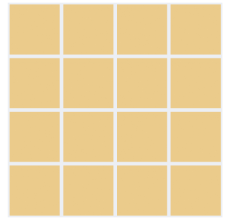
\includegraphics{images/4x4_start_board.PNG}
        \sethebrew
    \end{subfigure}%
    \begin{subfigure}{.5\textwidth}
        \unsethebrew
        \caption{\R{לחיצה על משבצת מסומנת}}
        \centering
        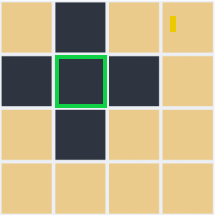
\includegraphics{images/4x4_press.PNG}
        \sethebrew
    \end{subfigure}%
\end{figure}

נבחין כי המשחק 
$4x4$
מתחיל במצב
\L{(a)}.
\\
בלוח 
\L{(b)}
נתאר מצב בו לחצו על משבצת המסומנת, בירוק
כל המשבצות השכנות והיא משנות מצבן, היות ומצב של כולן היה דלוקות לכן הן נכבו

המשחק במקור היה צעצוע אלקטרוני על לוח 
$5x5$
ששוחרר ב 
$1995$.
\\
המשחק יכול להראות פשוט אבל כפי שתואר
במאמר
\cite{B1}
\L{"devilish invention"}.
\\
קיים קושי רב בלמצוא שיטה לפתרון אינטואיטיבי, הקושי של משחק מתבלט בשאלה כיצד כדי להתחיל את המשחק?
\\
בנוסף אציין מניסיון האישי שהמשחק קשה כבר 
על לוח 
$5x5$
ולרוב אנשים שמשחקים אותו מכירים מצבים על הלוח שיודע עליהם משם את הפתרון.

פרויקט זה באה בעקבות הקושי של המשחק
והניסוי להציע שיטות לפתרון, בעקבות ניסיונות עלו
נעזרנו במספר רב של כלים מתמטיים מתקדמים.
\\
אחת המטרות במחקר למצוא הסבר לתופעות במשחק שנתקלנו.

נציין כי קיימים עוד המון שאלות שמשחק מעלה ולא לכולם קיים פתרון,
נשמח בפרויקט זה פתרון לכמה מהשאלות שעולות.
\\
חוץ מאתגר של המשחק עצמו קיים אתגר מתמטי שנרצה בפרויקט זה להציג ולהעניין.


\subsection{ משחק האורות על גרף}
אחרי שכללי המשחק על לוח הובנו אפשר לנסות להכליל את המשחק כמשחק על גרף.
\\
קיימים הרבה סיבות בהם תירצה להגדיר את הבעיה על מבנה כללי שכזה:

\begin{enumerate}
    \item 
    ככול שמבנה כללי יותר תאוריה שאתה מפתח מתאימה ליותר בעיות.
    \item 
    קיימת תאוריה רחבה שפותחה על גרפים ואתכן שנעזר בחלק
    מהטענות מהתאורה שכזה.
    \item 
    מבליט את מהות הבעיה והגדרה הבסיסית ביותר של המשחק.
\end{enumerate}

ארצה להתייחס לנקודה אחרונה, החשיבות הגדולה שאפשר לתאר את הבעיה של משחק
כאוסף של כללים על גרף, מרכזת אותנו לבעיה ובסופו של דבר כשנראה את שיטה למציאת
הפתרון, השיטה עצמה תזכיר לנו מיד את הייצוג הגרפי.

כדי לתאר את משחק האורות על גרף נשתמש באותם כללים שהגדרנו פרט לעובדה
שצמתים הם הלחצנים או המשבצות במקרה של הלוח
וכל לחיצה הופכת את המצב של הצומת והשכנים שלה.
\\
נזכיר כי צמתים שכנים הם צמתים שיש
קשת ביניהם.

נציין כי כאשר כל צומת יכולה להיות בשתי מצבים,
דלוקה או כבויה המטרה היא לעבור מכל הצמתים במצב מסוים דלוק למצב אחר כבוי.
\\
העובדה שמצב התחלתי הינו דלוק או כבוי אינה תשנה את המשחק עלה רק לאיזה מצב סופי צריך לעבור
לכבוי או דלוק.

נמחיש זאת על דוגמה:
\begin{figure}[h]
    \begin{subfigure}{.5\textwidth}
        \unsethebrew
        \caption{\R{מצב התחלתי}}
        \centering
        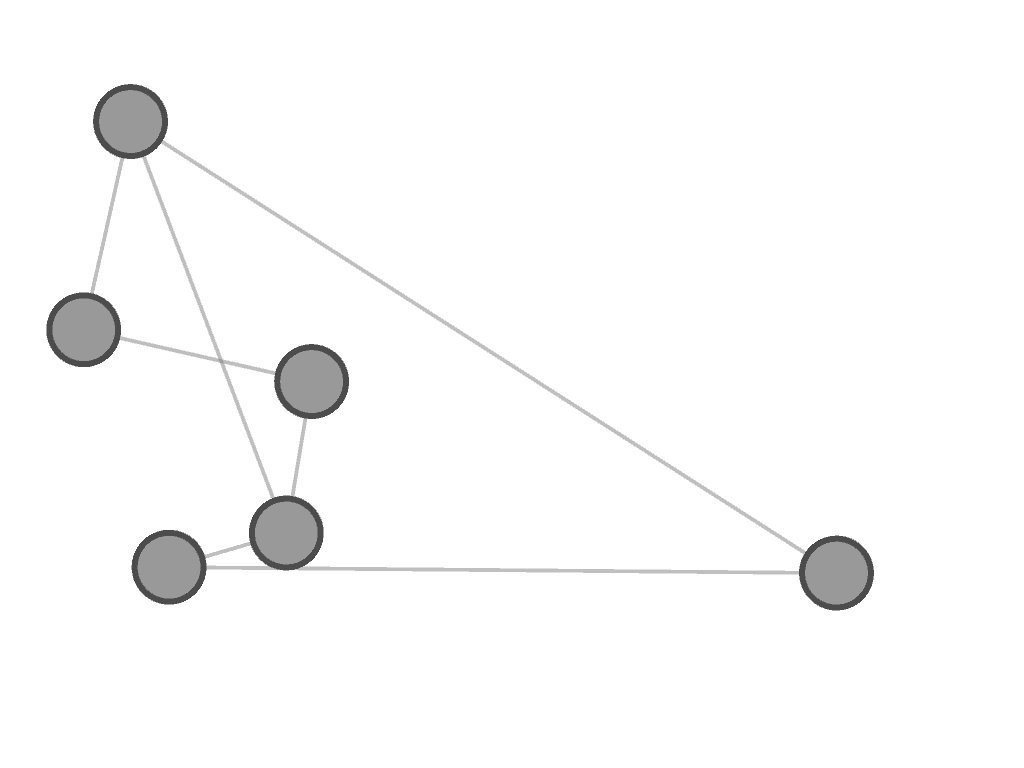
\includegraphics[width=\textwidth,height=\textheight,keepaspectratio]{images/graph_start_board.png}
        \sethebrew
    \end{subfigure}%
    \begin{subfigure}{.5\textwidth}
        \unsethebrew
        \caption{\R{לחיצה על משבצת מסומנת}}
        \centering
        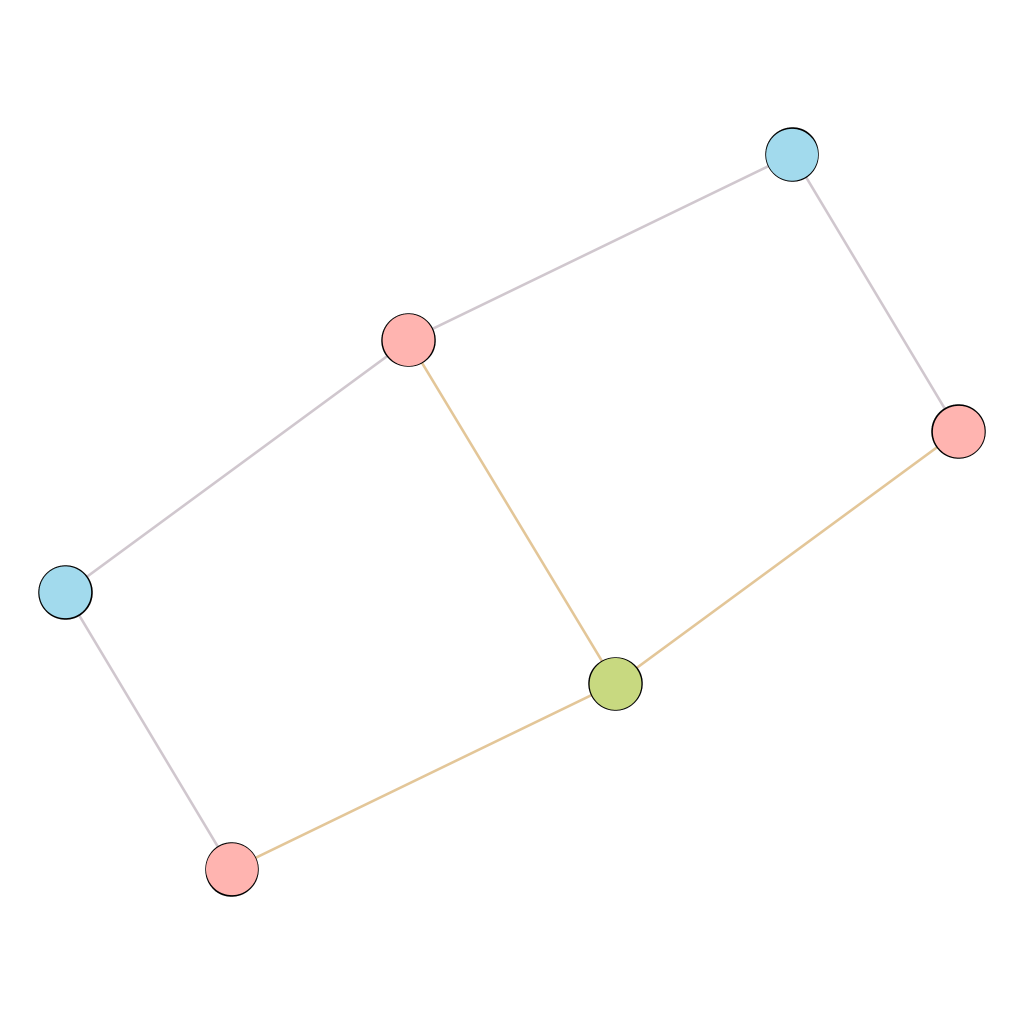
\includegraphics[width=\textwidth,height=\textheight,keepaspectratio]{images/graph_press.png}
        \sethebrew
    \end{subfigure}%
\end{figure}

על גרף התחלתי
\L{(a)}
ניתן לראות
$6$
קודקודיים
צבועים באפור ומטרה לצבוע את כולם לצהוב.
\\
בשלב 
\L{(b)}
מציגים  לחיצה על צומת ירוקה היא ושכניה נצבעים בצהוב.

\begin{comm}
    בפועל צומת ירוקה גם נצבעת לצהוב צביעה לירוק נועדה להדגשה על מי נלחץ
\end{comm}

משחק על גרף הינה הכללה  של משחק על לוח כלומר, כל משחק 
לוח ניתן לתאר בעזרת משחק על גרף.

נמחיש זאת על דוגמה:

ניקח לוח למשל
$2 \times 3$
נמספר את המשבצות כמו באיור
\ref{2x3_board}

\begin{figure}[ht]
    \unsethebrew
    \caption{
        \R{לוח
        $2 \times 3$
        }
    }
    \centering
    \label{2x3_board}
    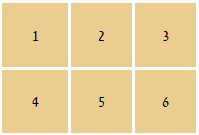
\includegraphics[width=0.5\textwidth,height=0.5\textheight,keepaspectratio]{images/2x3_board.PNG}
    \sethebrew
\end{figure}

כדי לתאר את הלוח על על משחק גרף נשתמש בשני הכללים הבאים:

\begin{enumerate}
    \item 
    כל משבצת על משחק לוח נהפוך לנקודה.
    \item 
    כל זוג משבצות סמוכות על לוח נחבר את נקודות בקו
\end{enumerate}

הגרף שנקבל עבור לוח באיור
\ref{2x3_board}
מתואר באיור
\ref{2x3_graph}

\begin{figure}[ht]
    \unsethebrew
    \caption{
        \R{גרף
        $2 \times 3$
        }
    }
    \centering
    \label{2x3_graph}
    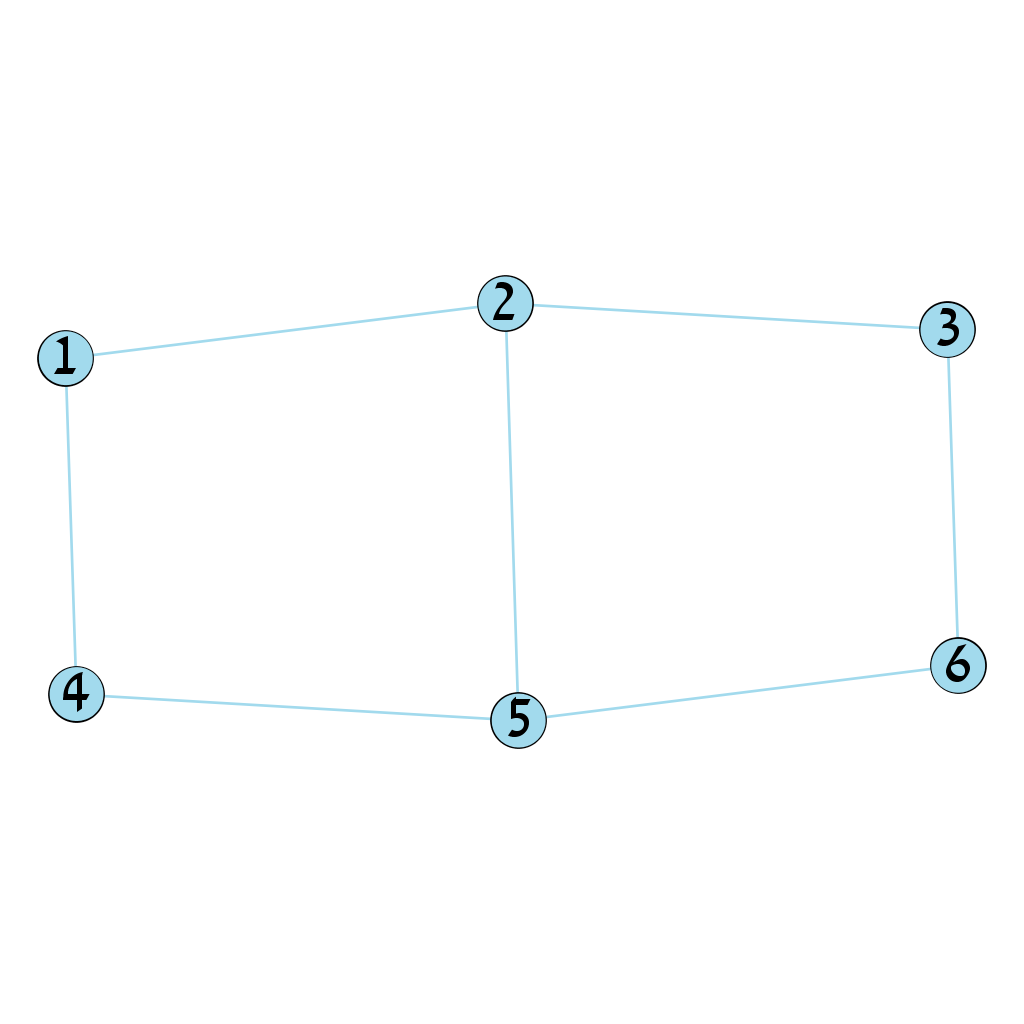
\includegraphics[width=0.5\textwidth,height=0.5\textheight,keepaspectratio]{images/2x3_graph.png}
    \sethebrew
\end{figure}

נשים לב שלגרף בו יש צומת אם יותר מ
$4$
שכנים לא ניתן לתאר לוח שכזה כיוון שלכל היות במשחק על לוח
לכל משבצת יש לכל יותר 
$4$
משבצות סמוכות.

לכן לסיכום אפשר למדל כל משחק לוח על משחק גרף שמייצג אותו אבל 
ההפך זה לא נכון.

\newpage

\section{ אלגוריתם למציאת פתרון}
לפני שנציא שיטה לפתרון נציין מדוע  נציין מדוע קיים הצורך לחפש פיתרון
אחת הסיבות המרכזיות שמספר אפשרויות לנסיון גדולותת מהר

\subsection{פתרון בעזרת שיטה הספרדית}
% TODO: 

\section{הוכחת  קיום פתרון עבור כל גרף}
% TODO:

\subsection{מספר הפתרונות עבור כל גרף}
% TODO:

\section{פתרון מינימלי עבור לוחות מלבניים}
% TODO:

\section{תוצאות ומסקנות}
% TODO:

\section{נספחים}
% TODO:

%----------------------------------------------------------------------------------------
%   רשימת מקורות
%----------------------------------------------------------------------------------------
\section{} %ביבליוגרפיה
\begin{thebibliography}{99}
\unsethebrew
\bibitem{B1} ALL LIGHTS AND LIGHTS OUT
An investigation among lights and shadows by
SUMA magazine’s article by Rafael Losada
Translated from Spanish by Ángeles Vallejo
\sethebrew

\end{thebibliography}

\end{document} 
